\documentclass[lualatex,paper=a4,fontsize=9pt]{jlreq}

\usepackage{amsmath,amssymb}
\usepackage{booktabs}
\usepackage{geometry}
\usepackage{graphicx}
\usepackage{tikz}
\usetikzlibrary{arrows.meta,positioning,fit,calc,backgrounds}

\geometry{margin=14mm}
\pagestyle{empty}

\title{TALE-SD accepted-pulse graph GNN with waveform features}
\author{}
\date{}

\begin{document}
\maketitle
\vspace{-8mm}

\section{目的}

TALE-SDは検出器配置が不均一であり、規則格子を仮定するCNNだけでは検出器配置の情報を自然に扱えない。
本モデルでは、各検出器を任意のIDとして扱うのではなく、物理的に意味のある量だけを入力する。
具体的には、絶対位置、標高、イベント内の重心からの相対位置、局所的な検出器間隔、信号時刻、信号量、校正量、ノイズ量、accepted pulseに付随する上下層の波形情報、検出器間の時空間的なedgeを用いる。

ノードは、Ising/noise filtering後に残ったaccepted pulseに対応する。
各ノードには、通常の特徴量に加えて、上層/下層のraw pulse windowと、accepted pulse区間だけを時刻順に詰めたcompact traceを付与する。
これにより、ノイズ除去後のパルス列を直接使う場合と、周辺波形を含めて使う場合を同じモデル内で比較できる。

\begin{figure}[htbp]
  \centering
  \resizebox{\linewidth}{!}{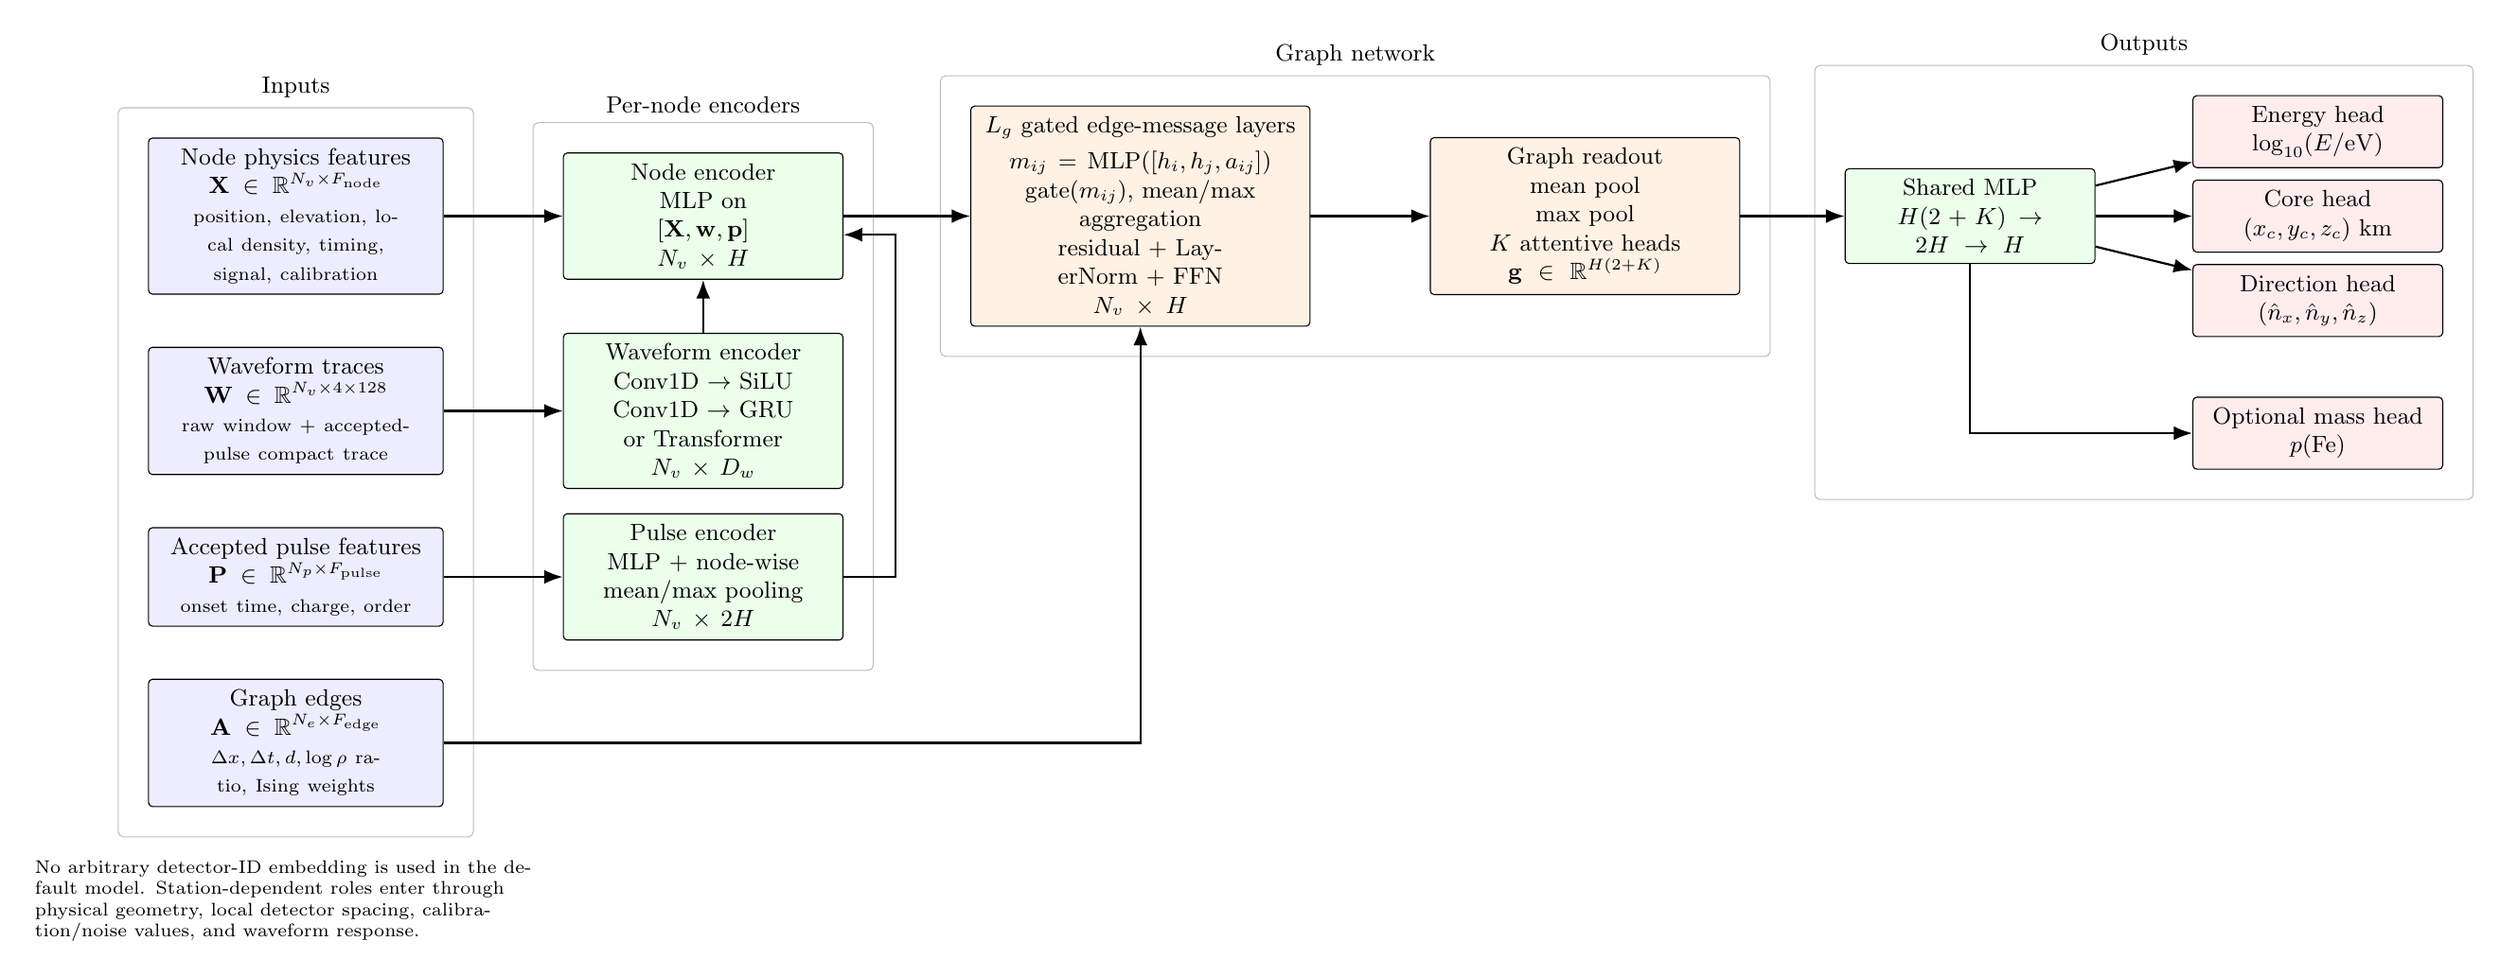
\begin{tikzpicture}[
  font=\small,
  box/.style={draw, rounded corners=1.5pt, align=center, minimum height=9mm, inner xsep=5pt, inner ysep=4pt},
  input/.style={box, fill=blue!7},
  enc/.style={box, fill=green!8},
  gnn/.style={box, fill=orange!10},
  output/.style={box, fill=red!7},
  note/.style={align=left, font=\scriptsize},
  arrow/.style={-{Latex[length=2.5mm]}, thick}
]

\node[input, text width=36mm] (x) {
  Node physics features\\
  $\mathbf{X}\in\mathbb{R}^{N_v\times F_{\mathrm{node}}}$\\
  \scriptsize position, elevation, local density, timing, signal, calibration
};
\node[input, text width=36mm, below=7mm of x] (w) {
  Waveform traces\\
  $\mathbf{W}\in\mathbb{R}^{N_v\times4\times128}$\\
  \scriptsize raw window + accepted-pulse compact trace
};
\node[input, text width=36mm, below=7mm of w] (p) {
  Accepted pulse features\\
  $\mathbf{P}\in\mathbb{R}^{N_p\times F_{\mathrm{pulse}}}$\\
  \scriptsize onset time, charge, order
};
\node[input, text width=36mm, below=7mm of p] (e) {
  Graph edges\\
  $\mathbf{A}\in\mathbb{R}^{N_e\times F_{\mathrm{edge}}}$\\
  \scriptsize $\Delta x,\Delta t,d,\log\rho$ ratio, Ising weights
};

\node[enc, text width=34mm, right=16mm of w] (wenc) {
  Waveform encoder\\
  Conv1D $\rightarrow$ SiLU\\
  Conv1D $\rightarrow$ GRU\\
  or Transformer\\
  $N_v\times D_w$
};
\node[enc, text width=34mm, right=16mm of p] (penc) {
  Pulse encoder\\
  MLP + node-wise\\
  mean/max pooling\\
  $N_v\times2H$
};
\node[enc, text width=34mm, right=16mm of x] (xenc) {
  Node encoder\\
  MLP on\\
  $[\mathbf{X},\mathbf{w},\mathbf{p}]$\\
  $N_v\times H$
};

\node[gnn, text width=42mm, right=17mm of xenc] (mp) {
  $L_g$ gated edge-message layers\\
  \vspace{1mm}
  $m_{ij}=\mathrm{MLP}([h_i,h_j,a_{ij}])$\\
  gate$(m_{ij})$, mean/max aggregation\\
  residual + LayerNorm + FFN\\
  $N_v\times H$
};

\node[gnn, text width=38mm, right=16mm of mp] (pool) {
  Graph readout\\
  mean pool\\
  max pool\\
  $K$ attentive heads\\
  $\mathbf{g}\in\mathbb{R}^{H(2+K)}$
};

\node[enc, text width=30mm, right=14mm of pool] (shared) {
  Shared MLP\\
  $H(2+K)\rightarrow2H\rightarrow H$
};

\node[output, text width=30mm, above right=0mm and 13mm of shared] (energy) {
  Energy head\\
  $\log_{10}(E/\mathrm{eV})$
};
\node[output, text width=30mm, right=13mm of shared] (core) {
  Core head\\
  $(x_c,y_c,z_c)$ km
};
\node[output, text width=30mm, below right=0mm and 13mm of shared] (dir) {
  Direction head\\
  $(\hat n_x,\hat n_y,\hat n_z)$
};
\node[output, text width=30mm, below=8mm of dir] (mass) {
  Optional mass head\\
  $p(\mathrm{Fe})$
};

\draw[arrow] (w) -- (wenc);
\draw[arrow] (p) -- (penc);
\draw[arrow] (x) -- (xenc);
\draw[arrow] (wenc.north) -- (xenc.south);
\draw[arrow] (penc.east) -- ++(7mm,0) |- ([yshift=-2.5mm]xenc.east);
\draw[arrow] (xenc) -- (mp);
\draw[arrow] (e) -| (mp);
\draw[arrow] (mp) -- (pool);
\draw[arrow] (pool) -- (shared);
\draw[arrow] (shared) -- (energy);
\draw[arrow] (shared) -- (core);
\draw[arrow] (shared) -- (dir);
\draw[arrow] (shared) |- (mass);

\node[note, below=6mm of e, text width=70mm] (idnote) {
  No arbitrary detector-ID embedding is used in the default model. Station-dependent roles enter through physical geometry, local detector spacing, calibration/noise values, and waveform response.
};

\begin{scope}[on background layer]
  \node[draw=gray!50, rounded corners=2pt, fit=(x)(w)(p)(e), inner sep=4mm, label={[font=\small]above:Inputs}] {};
  \node[draw=gray!50, rounded corners=2pt, fit=(wenc)(penc)(xenc), inner sep=4mm, label={[font=\small]above:Per-node encoders}] {};
  \node[draw=gray!50, rounded corners=2pt, fit=(mp)(pool), inner sep=4mm, label={[font=\small]above:Graph network}] {};
  \node[draw=gray!50, rounded corners=2pt, fit=(shared)(energy)(core)(dir)(mass), inner sep=4mm, label={[font=\small]above:Outputs}] {};
\end{scope}

\end{tikzpicture}
}
  \caption{General TALE-SD waveform GNN. Detector ID is not used as a physics input. Detector-dependent meaning is represented by physical station coordinates, elevation, local array density, calibration/noise quantities, accepted-pulse time traces, and graph connectivity.}
  \label{fig:model_architecture}
\end{figure}

\section{今回の学習モデル}

図\ref{fig:concrete_training_model}は、\texttt{scripts/run\_waveform\_large\_training.sh}のdefault設定で今から学習するモデルを、具体的な次元と層の値を入れて書いたものである。
主な設定は、physics architecture、CNN--GRU waveform encoder、hidden dimension $H=192$、message-passing layer数 $L_g=5$、readout head数 $K=4$である。
任意のdetector-ID embeddingは使わず、\texttt{DETECTOR\_EMBEDDING\_DIM=0}とする。
主入力はaccepted pulseをノードにしたグラフであり、波形は各pulse nodeに付く補助特徴量である。
ここでのCNNは検出器平面上のCNNではなく、各pulse nodeに付随する4 channel traceに対する1次元畳み込みである。

\clearpage
\begin{figure}[p]
  \centering
  \resizebox{!}{0.77\textheight}{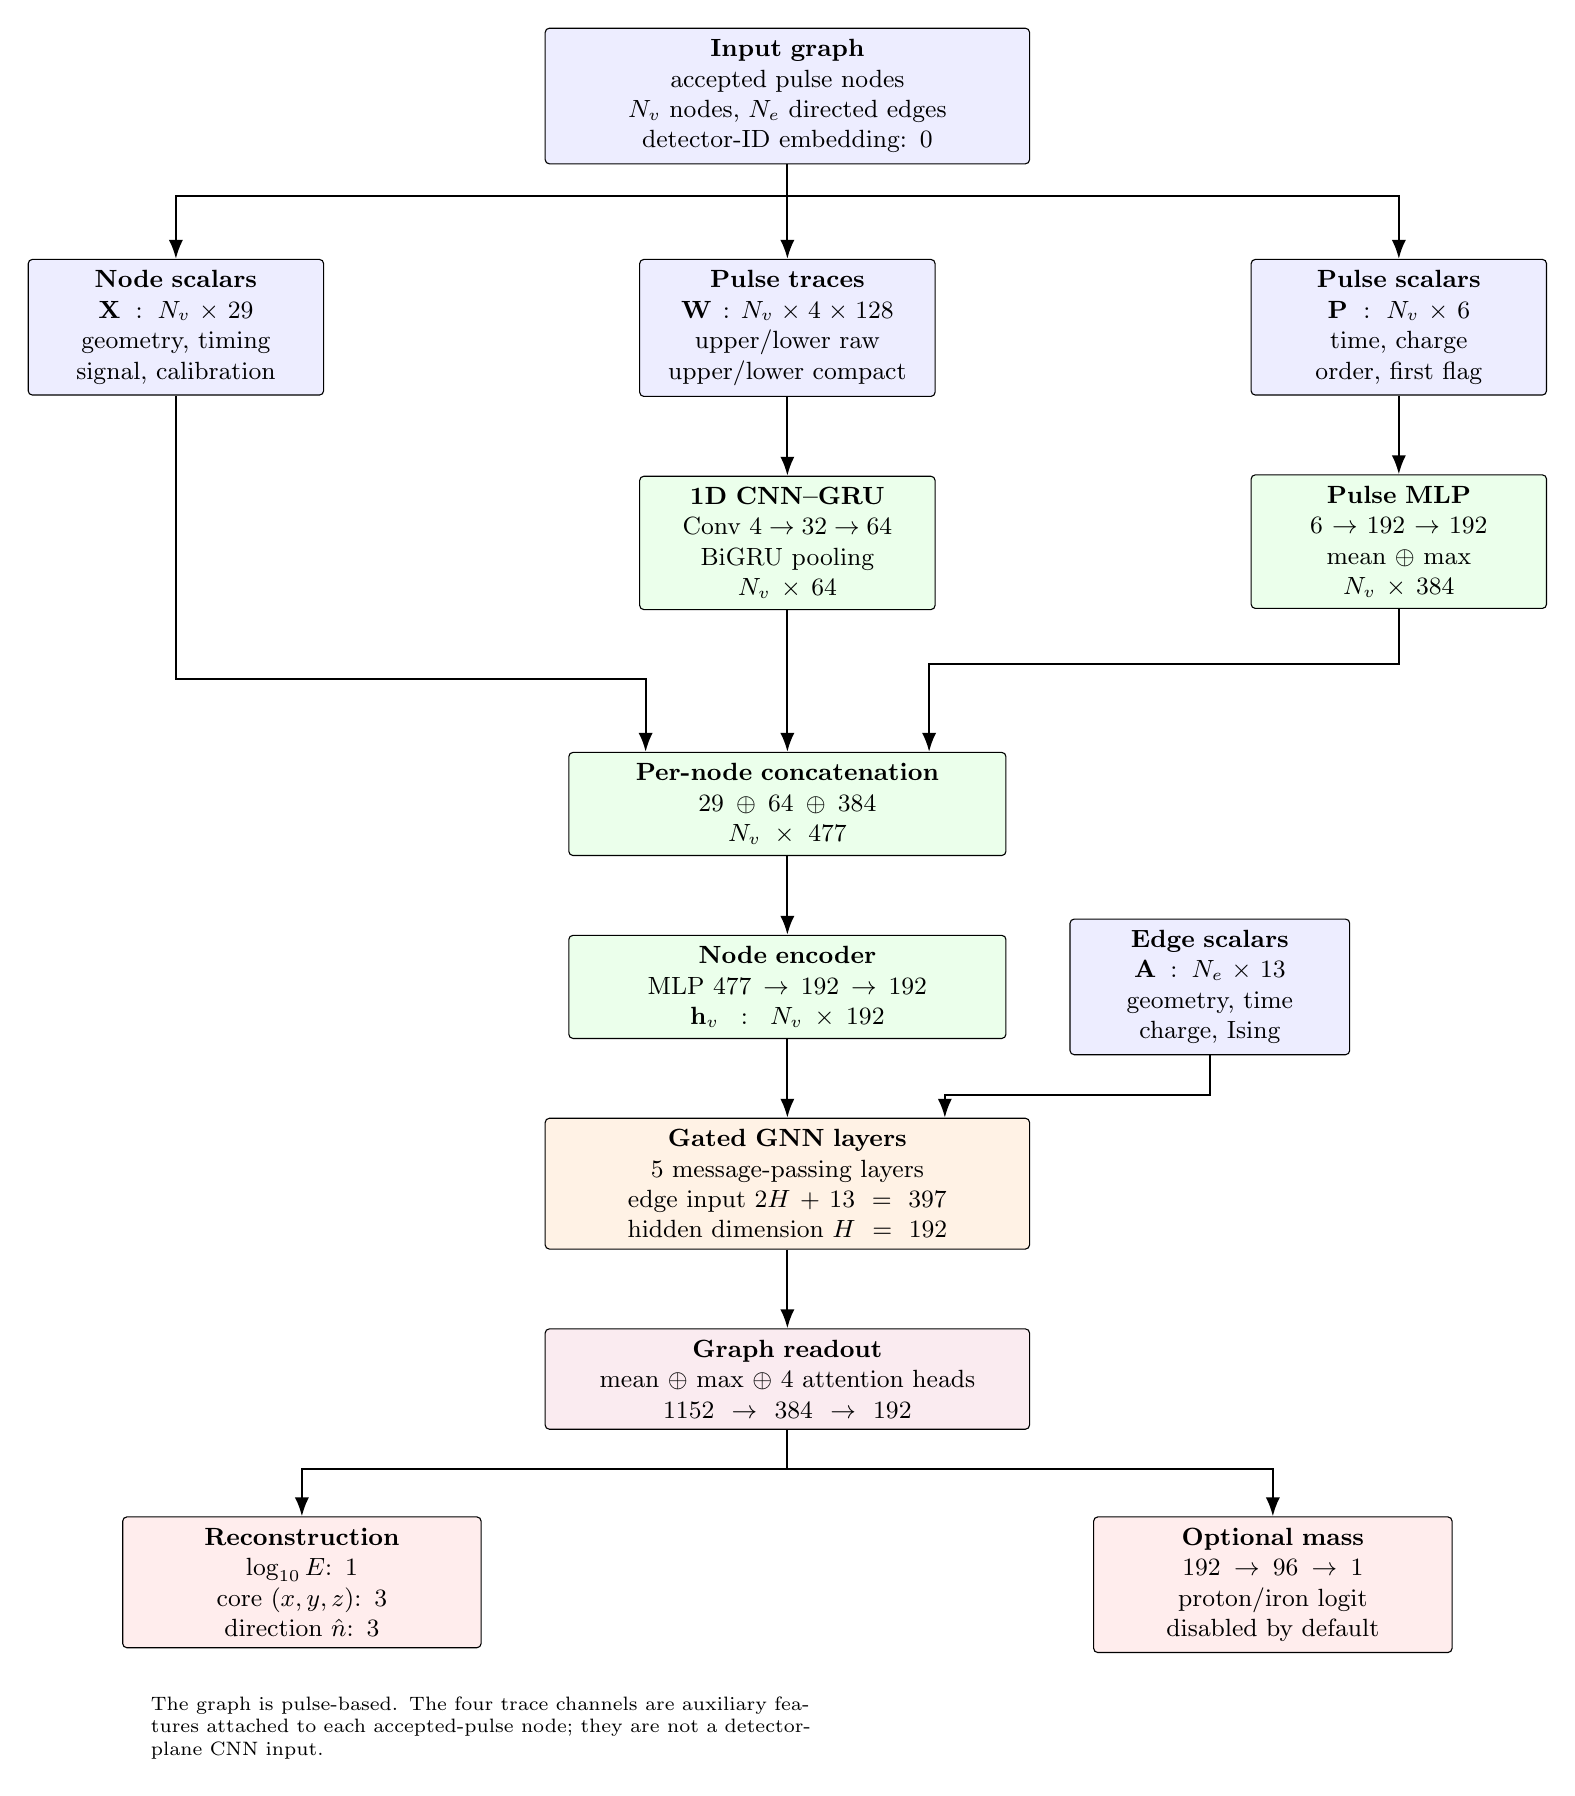
\begin{tikzpicture}[
  font=\small,
  box/.style={draw, rounded corners=1.5pt, align=center, inner xsep=5pt, inner ysep=4pt},
  input/.style={box, fill=blue!7},
  enc/.style={box, fill=green!8},
  gnn/.style={box, fill=orange!10},
  readout/.style={box, fill=purple!8},
  output/.style={box, fill=red!7},
  note/.style={align=left, font=\scriptsize},
  arrow/.style={-{Latex[length=2.4mm]}, thick}
]

\node[input, text width=58mm] (graph) at (0,0) {
  \textbf{Input graph}\\
  accepted pulse nodes\\
  $N_v$ nodes, $N_e$ directed edges\\
  detector-ID embedding: $0$
};

\node[input, text width=34mm, below left=12mm and 28mm of graph] (x) {
  \textbf{Node scalars}\\
  $\mathbf{X}:N_v\times29$\\
  geometry, timing\\
  signal, calibration
};
\node[input, text width=34mm, below=12mm of graph] (w) {
  \textbf{Pulse traces}\\
  $\mathbf{W}:N_v\times4\times128$\\
  upper/lower raw\\
  upper/lower compact
};
\node[input, text width=34mm, below right=12mm and 28mm of graph] (p) {
  \textbf{Pulse scalars}\\
  $\mathbf{P}:N_v\times6$\\
  time, charge\\
  order, first flag
};

\node[enc, text width=34mm, below=10mm of w] (wenc) {
  \textbf{1D CNN--GRU}\\
  Conv $4\!\to\!32\!\to\!64$\\
  BiGRU pooling\\
  $N_v\times64$
};
\node[enc, text width=34mm, below=10mm of p] (penc) {
  \textbf{Pulse MLP}\\
  $6\!\to\!192\!\to\!192$\\
  mean $\oplus$ max\\
  $N_v\times384$
};

\node[enc, text width=52mm, below=18mm of wenc] (concat) {
  \textbf{Per-node concatenation}\\
  $29\oplus64\oplus384$\\
  $N_v\times477$
};
\node[enc, text width=52mm, below=10mm of concat] (nenc) {
  \textbf{Node encoder}\\
  MLP $477\!\to\!192\!\to\!192$\\
  $\mathbf{h}_v:N_v\times192$
};

\node[input, text width=32mm, right=8mm of nenc] (edge) {
  \textbf{Edge scalars}\\
  $\mathbf{A}:N_e\times13$\\
  geometry, time\\
  charge, Ising
};

\node[gnn, text width=58mm, below=10mm of nenc] (mp) {
  \textbf{Gated GNN layers}\\
  $5$ message-passing layers\\
  edge input $2H+13=397$\\
  hidden dimension $H=192$
};

\node[readout, text width=58mm, below=10mm of mp] (readout) {
  \textbf{Graph readout}\\
  mean $\oplus$ max $\oplus$ $4$ attention heads\\
  $1152\!\to\!384\!\to\!192$
};

\node[output, text width=42mm, below left=11mm and 8mm of readout] (reco) {
  \textbf{Reconstruction}\\
  $\log_{10}E$: $1$\\
  core $(x,y,z)$: $3$\\
  direction $\hat{n}$: $3$
};
\node[output, text width=42mm, below right=11mm and 8mm of readout] (mass) {
  \textbf{Optional mass}\\
  $192\!\to\!96\!\to\!1$\\
  proton/iron logit\\
  disabled by default
};

\draw[arrow] (graph.south) -- ++(0,-4mm) -| (x.north);
\draw[arrow] (graph.south) -- (w.north);
\draw[arrow] (graph.south) -- ++(0,-4mm) -| (p.north);
\draw[arrow] (w) -- (wenc);
\draw[arrow] (p) -- (penc);
\draw[arrow] (x.south) -- ++(0,-36mm) -| ([xshift=-18mm]concat.north);
\draw[arrow] (wenc.south) -- (concat.north);
\draw[arrow] (penc.south) -- ++(0,-7mm) -| ([xshift=18mm]concat.north);
\draw[arrow] (concat) -- (nenc);
\draw[arrow] (nenc) -- (mp);
\draw[arrow] (edge.south) -- ++(0,-5mm) -| ([xshift=20mm]mp.north);
\draw[arrow] (mp) -- (readout);
\draw[arrow] (readout.south) -- ++(0,-5mm) -| (reco.north);
\draw[arrow] (readout.south) -- ++(0,-5mm) -| (mass.north);

\node[note, below=5mm of reco.south east, text width=84mm, anchor=north] {
  The graph is pulse-based.  The four trace channels are auxiliary features attached to each accepted-pulse node; they are not a detector-plane CNN input.
};

\end{tikzpicture}
}
  \caption{Concrete model used by the default waveform training script. Dimensions are shown for the run configuration used before launching the next DST export and training.}
  \label{fig:concrete_training_model}
\end{figure}
\clearpage

\begin{table}[htbp]
  \centering
  \caption{Concrete default values for the next waveform training run.}
  \begin{tabular}{lll}
    \toprule
    Quantity & Value & Meaning \\
    \midrule
    $F_{\mathrm{node}}$ & 29 & geometry, local array density, timing, signal, calibration/noise \\
    $F_{\mathrm{edge}}$ & 13 & relative geometry, timing, signal ratio, Ising weights \\
    $F_{\mathrm{pulse}}$ & 6 & pulse time, charge proxy, pulse order, first-pulse flag \\
    waveform tensor & $4\times128$ & upper/lower raw window and upper/lower compact accepted-pulse trace \\
    waveform embedding & 64 & CNN--GRU output per pulse-node \\
    node encoder input & 477 & $29+64+2\times192+0$ \\
    graph hidden dimension & 192 & node state dimension in message passing \\
    message-passing layers & 5 & gated edge-message layers \\
    readout dimension & 1152 & $192\times(2+4)$ from mean, max, and 4 attentive heads \\
    reconstruction output & 7 & $\log_{10}E$, core $(x,y,z)$, direction $(n_x,n_y,n_z)$ \\
    optimizer & AdamW & learning rate $3\times10^{-4}$, weight decay $10^{-4}$ \\
    split & source-stratified & validation $10\%$, test $20\%$ \\
    \bottomrule
  \end{tabular}
\end{table}

\section{グラフ定義}

グラフ化は\texttt{../coincidence\_analysis}で作成済みのIsing graph定義を使う。
このGNNでも、ノードはSD番号そのものではなく、Ising/noise filtering後に残ったaccepted pulseである。
同じ検出器に複数のaccepted pulseが残る場合は、その検出器から複数ノードが作られる。
edgeは異なる検出器のpulse node間にのみ張り、距離、時刻差、信号量、Ising-style weightをedge featureとして持たせる。

\begin{figure}[htbp]
  \centering
  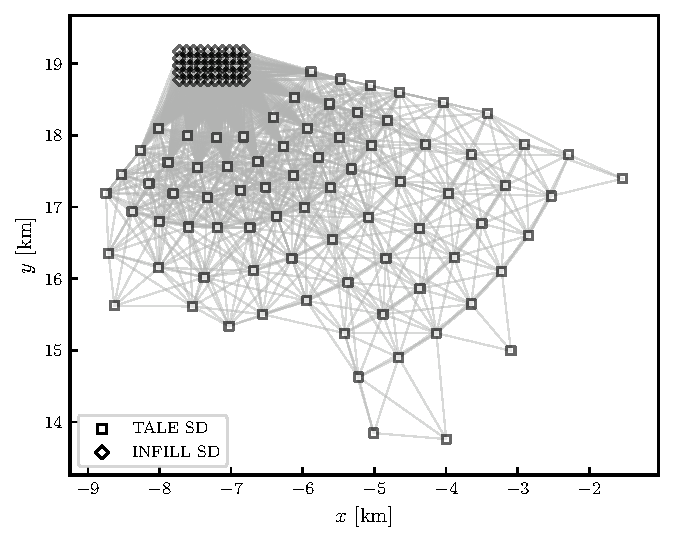
\includegraphics[width=0.70\linewidth]{fig/ising_edge_candidate_graph.pdf}
  \caption{Ising edge candidate graph copied from \texttt{../coincidence\_analysis}. This is the layout-aware detector-pair graph used as the basis of the pulse-level GNN edge definition.}
  \label{fig:ising_edge_candidate_graph}
\end{figure}

\begin{figure}[htbp]
  \centering
  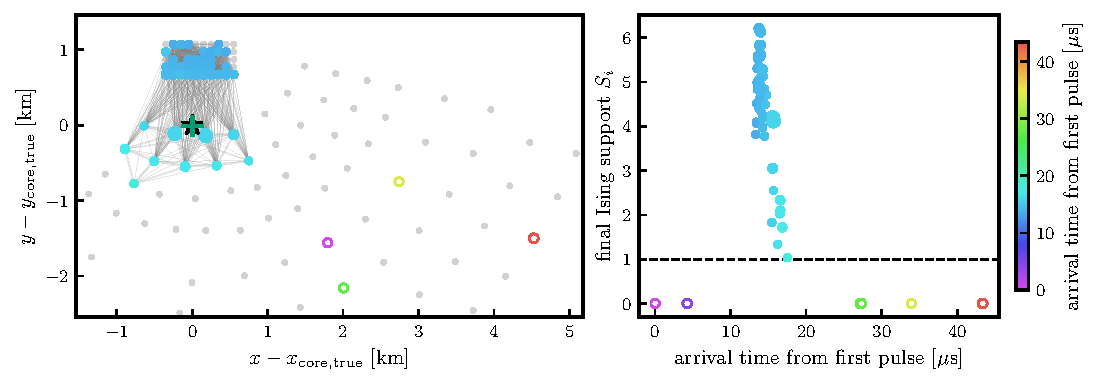
\includegraphics[width=0.92\linewidth]{fig/mc_ising_filter_event.pdf}
  \caption{Representative pulse-candidate graph and Ising selection copied from \texttt{../coincidence\_analysis}. The GNN uses the same pulse-level idea: accepted pulse candidates become graph nodes, and local space-time relations become edges.}
  \label{fig:mc_ising_filter_event}
\end{figure}

\vspace{-2mm}
\begin{table}[htbp]
  \centering
  \caption{Main tensors and dimensions. $N_v$ is the number of accepted pulse-nodes in one shower graph, $N_e$ is the number of directed graph edges, $L=128$ is the trace length, $H$ is the graph hidden dimension, $D_w$ is the waveform embedding dimension, and $K$ is the number of attentive readout heads.}
  \resizebox{\linewidth}{!}{%
  \begin{tabular}{@{}lll@{}}
    \toprule
    Tensor & Dimension & Content \\
    \midrule
    $\mathbf{X}$ & $N_v \times F_{\mathrm{node}}$ &
    position, elevation, local detector density, timing, signal size, calibration/noise \\
    $\mathbf{W}$ & $N_v \times 4 \times 128$ &
    upper/lower raw pulse windows and upper/lower accepted-pulse compact traces \\
    $\mathbf{P}$ & $N_p \times F_{\mathrm{pulse}}$ &
    accepted-pulse time, charge, pulse order, first-pulse flag \\
    $\mathbf{A}$ & $N_e \times F_{\mathrm{edge}}$ &
    relative position, distance, time difference, charge ratio, Ising edge weights \\
    $\mathbf{h}_v$ & $N_v \times H$ &
    node embeddings after waveform, pulse, and graph message passing \\
    $\mathbf{g}$ & $H(2+K)$ &
    graph-level mean, max, and attentive pooling vector \\
    \bottomrule
  \end{tabular}%
  }
\end{table}

\vspace{-1mm}
\begin{table}[htbp]
  \centering
  \caption{Layer definitions used in the default waveform model.}
  \resizebox{\linewidth}{!}{%
  \begin{tabular}{@{}lll@{}}
    \toprule
    Block & Operation & Output \\
    \midrule
    Waveform encoder &
    Conv1D $\rightarrow$ SiLU $\rightarrow$ Conv1D $\rightarrow$ CNN--GRU or Transformer pooling &
    $N_v \times D_w$ \\
    Pulse encoder &
    MLP on accepted-pulse features, then node-wise mean/max aggregation &
    $N_v \times 2H$ \\
    Node encoder &
    MLP on $[\mathbf{X}, \mathbf{w}, \mathbf{p}]$ &
    $N_v \times H$ \\
    Message passing &
    $L_g$ gated edge-message layers with residual normalization &
    $N_v \times H$ \\
    Readout &
    mean pooling, max pooling, and $K$ attentive pooling heads &
    $H(2+K)$ \\
    Reconstruction heads &
    shared MLP followed by energy, core, and direction heads &
    $(\log_{10}E,\ x_c,y_c,z_c,\ \hat{n}_x,\hat{n}_y,\hat{n}_z)$ \\
    Mass head &
    optional binary head for proton/iron comparison &
    $p({\mathrm{Fe}})$ \\
    \bottomrule
  \end{tabular}%
  }
\end{table}

\section{Baseline result}

図\ref{fig:baseline_learning_curve}--\ref{fig:baseline_species_energy}は、既存graphで学習したbaseline GNNのtest結果である。
このbaselineは波形trace encoderをまだ使っていないため、次の長時間学習で比較すべき下限性能として扱う。
波形付きモデルの学習後は、同じ形式の図をここに差し替える。

\begin{figure}[htbp]
  \centering
  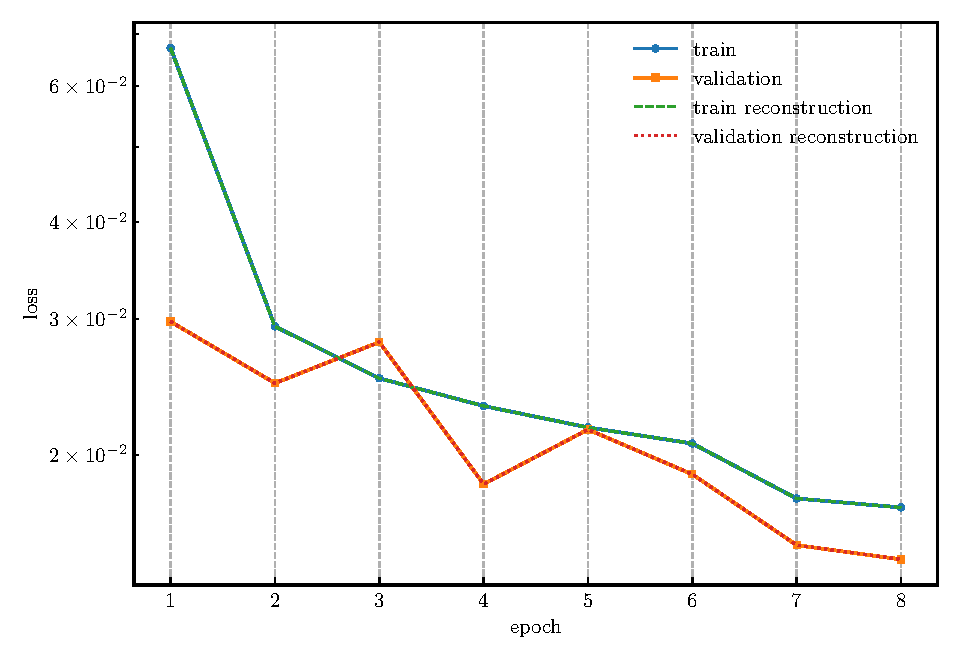
\includegraphics[width=0.72\linewidth]{fig/results/baseline_learning_curve.pdf}
  \caption{Baseline training and validation losses.}
  \label{fig:baseline_learning_curve}
\end{figure}

\begin{figure}[htbp]
  \centering
  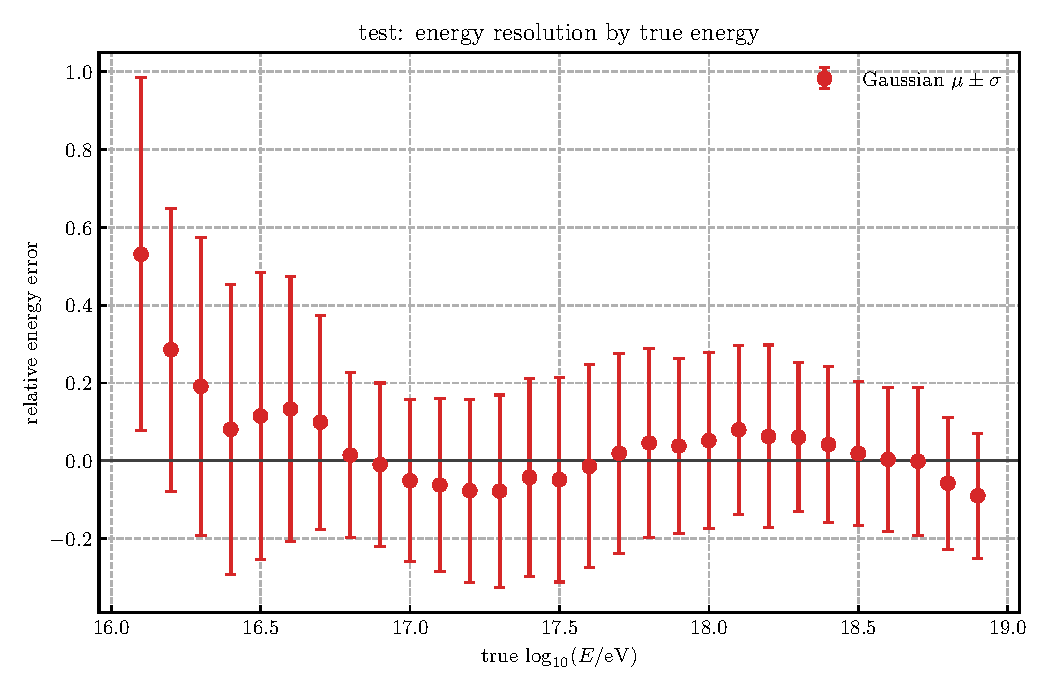
\includegraphics[width=0.78\linewidth]{fig/results/baseline_test_energy_resolution_by_true_energy.pdf}
  \caption{Baseline energy bias and resolution as a function of true energy for the test set.}
  \label{fig:baseline_energy}
\end{figure}

\begin{figure}[htbp]
  \centering
  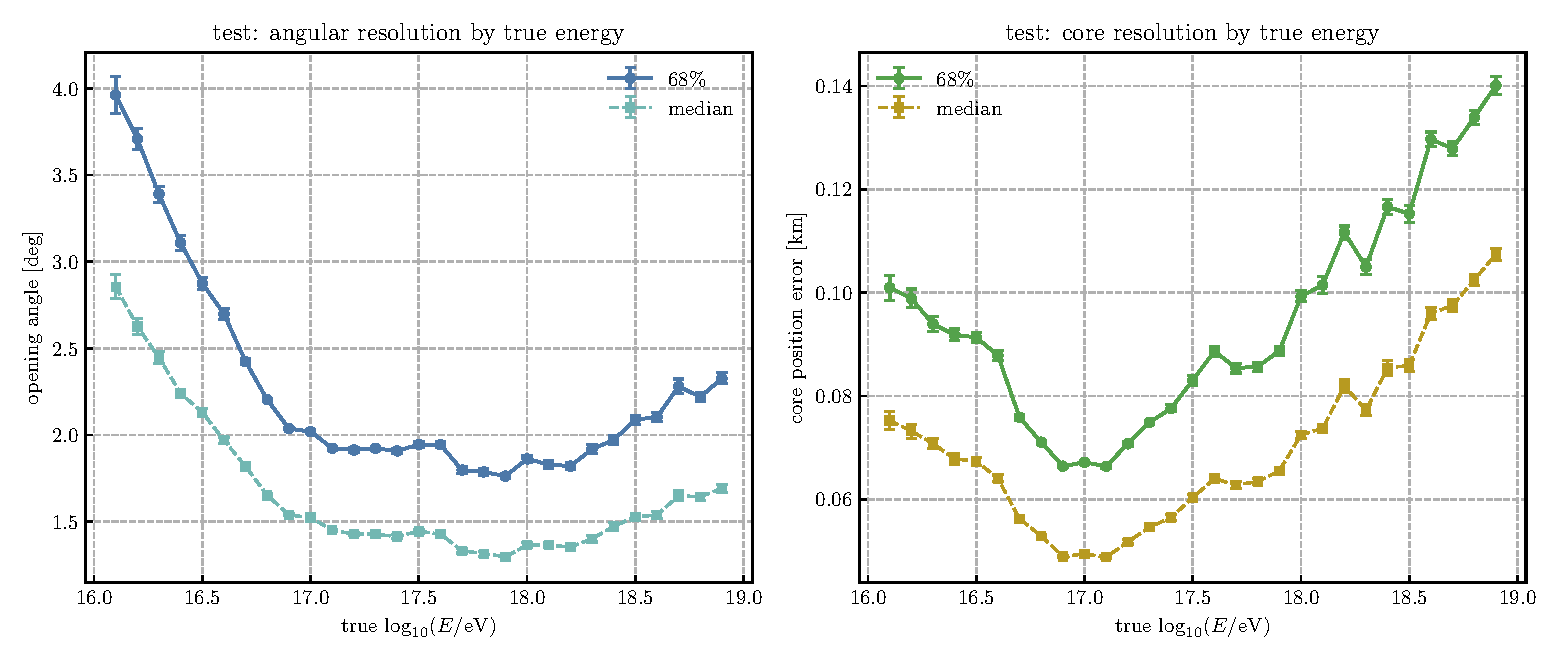
\includegraphics[width=0.82\linewidth]{fig/results/baseline_test_angular_core_resolution_by_true_energy.pdf}
  \caption{Baseline angular and core-position resolution as a function of true energy for the test set.}
  \label{fig:baseline_angle_core}
\end{figure}

\begin{figure}[htbp]
  \centering
  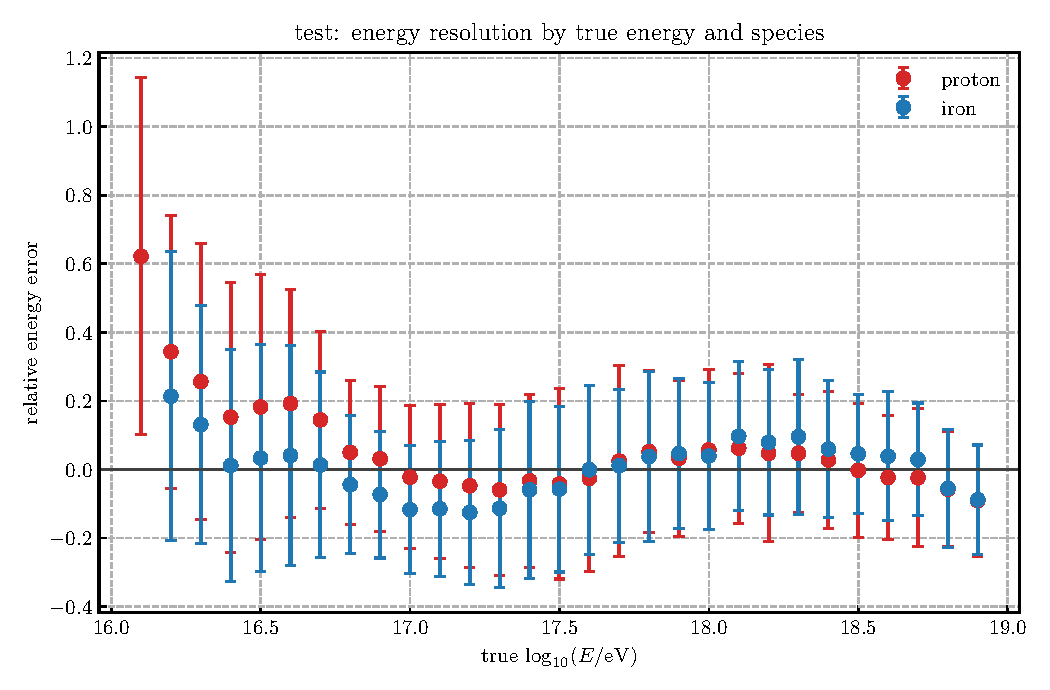
\includegraphics[width=0.78\linewidth]{fig/results/baseline_test_species_energy_resolution_by_true_energy.pdf}
  \caption{Baseline energy reconstruction split by primary species. Proton and iron are overlaid in the same panel.}
  \label{fig:baseline_species_energy}
\end{figure}

\end{document}
